\documentclass[10pt,a4paper,twocolumn]{article}

\usepackage[T1]{fontenc}
\usepackage[utf8]{inputenc}
\usepackage[english,brazil]{babel}
\usepackage{lmodern}
\usepackage{microtype}
\usepackage{geometry}
\usepackage{setspace}
\usepackage{graphicx}
\usepackage{booktabs}
\usepackage{tabularx}
\usepackage{array}
\usepackage{siunitx}
\usepackage[tablesonly,nomarkers,nolists,noheads]{endfloat}
\renewcommand{\efloatseparator}{\par\smallskip}
\usepackage{hyperref}
\usepackage{xcolor}
\usepackage[alf,abnt-emphasize=bf]{abntex2cite}

\geometry{top=2cm,bottom=2cm,left=1.8cm,right=1.8cm,columnsep=0.7cm}
\setstretch{1.02}
\setlength{\parindent}{0.7cm}
\setlength{\parskip}{0pt}
\hypersetup{
  colorlinks=true,
  linkcolor=black,
  citecolor=black,
  urlcolor=blue!50!black,
  pdftitle={Infraestrutura LoRaWAN para monitoramento térmico de instalações de produção animal},
  pdfauthor={Maria Fernanda Caetano}
}
\sisetup{output-decimal-marker={,}}

\newcommand{\keywords}[1]{\noindent\textbf{Palavras-chave:} #1}
\newcommand{\englishkeywords}[1]{\noindent\textbf{Keywords:} #1}

\title{\textbf{Infraestrutura LoRaWAN para monitoramento térmico de instalações de produção animal: projeto aplicado ao IFC Campus Araquari}}
\author{
  Maria Fernanda Caetano\\
  \small Bacharelado em Sistemas de Informação\\
  \small Instituto Federal Catarinense (IFC) -- Campus Araquari\\
  \small Disciplina de Projeto de Redes\\
  \small Orientador: Prof. Marcio Marcelo Piffer
}
\date{2026}

\begin{document}
\maketitle

\begin{abstract}
\noindent
O acompanhamento contínuo das condições ambientais em instalações de produção
animal pode apoiar o manejo, a pesquisa e a identificação precoce de situações de
desconforto térmico. Entretanto, a distribuição espacial das baias e a necessidade
de dispositivos alimentados por bateria dificultam o uso de redes convencionais.
Este artigo apresenta uma infraestrutura de Internet das Coisas
baseada em LoRaWAN para monitorar temperatura e, quando aplicável, umidade
relativa nos setores de bovinocultura, suinocultura e avicultura do Instituto
Federal Catarinense -- Campus Araquari. A pesquisa é aplicada, exploratória e de
natureza projetiva. Foram analisados os requisitos do ambiente, estudos sobre
redes LoRa em aplicações agropecuárias e os artefatos técnicos produzidos na
disciplina de Projeto de Redes. A solução especifica seis sensores Dragino
LHT65N-DC, um gateway Dragino LPS8N, comunicação em \SI{915}{\mega\hertz},
serviços gerenciados da AWS e aplicação web. O
fluxo proposto abrange aquisição, transmissão, persistência, visualização
histórica e geração de alertas. Entre as qualidades da proposta estão baixo
consumo nos pontos de sensoriamento, comunicação de longo alcance, cobertura de
áreas sem infraestrutura cabeada, centralização dos dados, separação dos
serviços de ingestão, processamento e armazenamento, segurança por identidade e
facilidade de expansão. Essas características podem reduzir inspeções manuais,
favorecer respostas rápidas a desvios térmicos e produzir históricos úteis ao
 manejo, ao ensino e à pesquisa. O custo inicial foi estimado em
R\$~2.977,00. Como não houve implantação física completa, os valores de
desempenho permanecem metas de aceitação, e não resultados experimentais.

\medskip
\keywords{LoRaWAN; Internet das Coisas; monitoramento ambiental; pecuária de precisão; redes de sensores.}
\end{abstract}

\selectlanguage{english}
\begin{abstract}
\noindent
Continuous monitoring of environmental conditions in animal production
facilities can support management, research, and early detection of thermal
discomfort. However, spatially distributed barns and battery-powered devices make
conventional networks difficult to deploy. This paper presents a
LoRaWAN-based Internet of Things infrastructure for monitoring temperature and,
where applicable, relative humidity in cattle, swine, and poultry facilities at
Instituto Federal Catarinense, Araquari Campus. This is an applied, exploratory,
and design-oriented study. Environmental requirements, research on agricultural
LoRa networks, and the technical artifacts produced in a Network Project course
were analyzed. The solution specifies six Dragino LHT65N-DC sensors, a Dragino
LPS8N gateway, \SI{915}{\mega\hertz} communication, managed AWS services, and a
web application. Its data flow covers acquisition, transmission, storage,
historical visualization, and alerts. The proposal combines low-power sensing,
long-range communication, centralized data, separated ingestion and storage
services, identity-based security, and scalability. These qualities can reduce
manual inspections, accelerate responses to thermal deviations, and provide
historical data for management, teaching, and research. The estimated initial
cost is BRL~2,977.00. Since a complete physical deployment was not performed,
performance values remain acceptance targets rather than experimental results.

\medskip
\englishkeywords{LoRaWAN; Internet of Things; environmental monitoring; precision livestock farming; sensor networks.}
\end{abstract}
\selectlanguage{brazil}

\section{Introdução}

A pecuária de precisão emprega sensores, conectividade e sistemas de informação
para transformar medições do ambiente e dos animais em apoio à decisão. Essa
abordagem complementa inspeções presenciais ao permitir séries históricas,
alertas e análise remota. Revisões recentes destacam a expansão de dispositivos
IoT na produção animal e, ao mesmo tempo, desafios relacionados à autonomia
energética, à conectividade rural e à validação em campo \cite{alves2025}.

Nas instalações do Instituto Federal Catarinense (IFC) -- Campus Araquari, os
setores de bovinocultura, suinocultura e avicultura atendem a atividades de
ensino, pesquisa e extensão. O levantamento realizado para este projeto
identificou que o acompanhamento térmico ocorre de forma manual ou sem uma
infraestrutura única de monitoramento contínuo. A ausência de dados centralizados reduz a capacidade
de observar variações ao longo do dia, construir históricos e reconhecer
rapidamente condições que demandem atenção dos responsáveis.

Redes de área ampla e baixa potência (\textit{Low-Power Wide-Area Networks} ---
LPWAN) são adequadas a esse cenário porque priorizam alcance e baixo consumo para
mensagens pequenas e esparsas. A tecnologia LoRa utiliza modulação por espectro
espalhado, enquanto LoRaWAN define a arquitetura de rede, o acesso ao meio, a
segurança e a comunicação entre dispositivos, gateways, servidor de rede e
aplicações \cite{macedo2023}. Estudos em ambientes agropecuários mostram que a
tecnologia pode integrar sensores e serviços remotos, mas também que obstáculos,
vegetação, distância e parâmetros de rádio influenciam a entrega de pacotes
\cite{fu2022,ting2024,ahmed2025}.

Diante disso, este trabalho tem como objetivo apresentar e analisar uma
uma infraestrutura LoRaWAN para monitoramento térmico das instalações de produção
animal do IFC Campus Araquari. As contribuições são: (i) consolidação dos
requisitos e da arquitetura; (ii) especificação do fluxo completo entre sensores
e aplicação; (iii) identificação de vantagens operacionais, econômicas e
acadêmicas; e (iv) análise de custo, riscos e escalabilidade.

\section{Fundamentação teórica}

\subsection{LoRa e LoRaWAN}

LoRa é uma tecnologia de camada física voltada à transmissão de baixa taxa de
dados em longas distâncias. O fator de espalhamento (\textit{spreading factor} ou
SF), a largura de banda, a taxa de codificação e a potência de transmissão
alteram o compromisso entre alcance, tempo no ar, robustez e consumo. Um SF maior
tende a elevar a sensibilidade do receptor, mas prolonga a ocupação do canal e o
gasto energético por mensagem. Por isso, os parâmetros devem ser definidos a
partir de medições no local, e não apenas do alcance nominal dos equipamentos
\cite{macedo2023,krizanovic2023}.

LoRaWAN adota uma topologia conhecida como \textit{star-of-stars}. Os
dispositivos finais não se associam exclusivamente a um gateway: uma transmissão
pode ser recebida por um ou mais gateways e encaminhada ao servidor de rede. Esse
servidor remove duplicidades, verifica a segurança e entrega a carga útil ao
servidor de aplicação \cite{macedo2023}. Para sensores que enviam dados
periodicamente e precisam economizar energia, a Classe A é a opção de menor
consumo, pois as janelas de recepção são abertas somente após uma transmissão.

LoRa não deve ser confundida com LoRaWAN. A primeira designa a interface de
rádio; a segunda, o protocolo e a arquitetura da rede. No projeto em estudo,
sensores e gateway utilizam LoRaWAN, e o gateway se conecta à infraestrutura IP
institucional ou, alternativamente, à rede celular.

\subsection{Monitoramento agropecuário com redes de sensores}

Aplicações agrícolas impõem um conjunto particular de restrições: grandes áreas,
pontos sem alimentação elétrica, umidade, poeira, interferências e obstáculos
variáveis. Em um sistema instalado em quatro galpões de produção leiteira,
\citeonline{fu2022} coletaram 6.140 conjuntos de dados e relataram taxa de perda
inferior a 1\% até \SI{604}{\meter}. O resultado demonstra viabilidade, mas não
pode ser transferido diretamente para outro local, pois propagação, antenas,
posicionamento e configuração diferem.

\citeonline{ahmed2025} observaram queda acentuada da razão de entrega de pacotes
sob vegetação, em comparação com campo aberto. De modo semelhante,
\citeonline{ting2024} verificaram influência significativa da distância, do
ambiente, da frequência e das condições meteorológicas. Esses achados justificam
o levantamento dos pontos e a validação de cobertura previstos neste projeto.

A autonomia também depende do intervalo de medição, corrente em repouso, SF,
tamanho do pacote e número de transmissões. Experimentos de
\citeonline{vaananen2022} indicam que compressão temporal e redução de
transmissões podem prolongar a vida da bateria; \citeonline{krizanovic2023}
destacam a importância de ajustar a carga útil e a taxa de transmissão. Assim,
temperaturas podem ser coletadas em frequência compatível com a dinâmica do
ambiente, evitando tráfego sem ganho informacional.

\section{Materiais e métodos}

O trabalho caracteriza-se como pesquisa aplicada, exploratória e de natureza
projetiva. O objeto não é a comparação experimental de protocolos, mas o
desenvolvimento de uma solução de rede para uma necessidade institucional. O
procedimento foi organizado em cinco etapas:

\begin{enumerate}
  \item análise dos setores de bovinocultura, suinocultura e avicultura e
  identificação dos pontos de monitoramento;
  \item levantamento de requisitos funcionais, não funcionais e restrições;
  \item revisão de 21 documentos-base sobre LoRa, LoRaWAN, IoT, monitoramento
  agropecuário, energia e propagação;
  \item elaboração da topologia física e lógica, especificação de equipamentos,
  orçamento, riscos e critérios de qualidade;
  \item consolidação dos artefatos de gerenciamento e do memorial descritivo
  produzidos durante o desenvolvimento do projeto na disciplina.
\end{enumerate}

Os requisitos funcionais considerados foram coleta periódica de temperatura,
recepção pelo gateway, persistência em banco de dados, consulta ao histórico,
visualização em aplicação web e geração de alertas. Os requisitos não funcionais
incluíram baixo consumo, operação remota, disponibilidade, integridade,
segurança, expansibilidade e interface responsiva.

A seleção dos componentes considerou compatibilidade com a faixa de
\SI{915}{\mega\hertz}, suporte a LoRaWAN, proteção para ambiente agropecuário,
autonomia, número de canais do gateway, disponibilidade e custo. A análise de
viabilidade foi documental: as metas de qualidade foram confrontadas com a
arquitetura e com resultados da literatura. Portanto, números não medidos no
campus são apresentados explicitamente como metas, nunca como resultados de
campo.

\section{Arquitetura proposta}

\subsection{Topologia e fluxo de dados}

A Figura~\ref{fig:arquitetura} apresenta a arquitetura consolidada. Seis nós
sensores são distribuídos entre os três setores. As mensagens são transmitidas ao
gateway LPS8N, que atua como ponte transparente entre o enlace LoRaWAN e a rede
IP. O tráfego segue para os serviços hospedados em nuvem, onde ocorre o
processamento, a persistência e a disponibilização para a aplicação web.

\begin{figure*}[t]
\centering
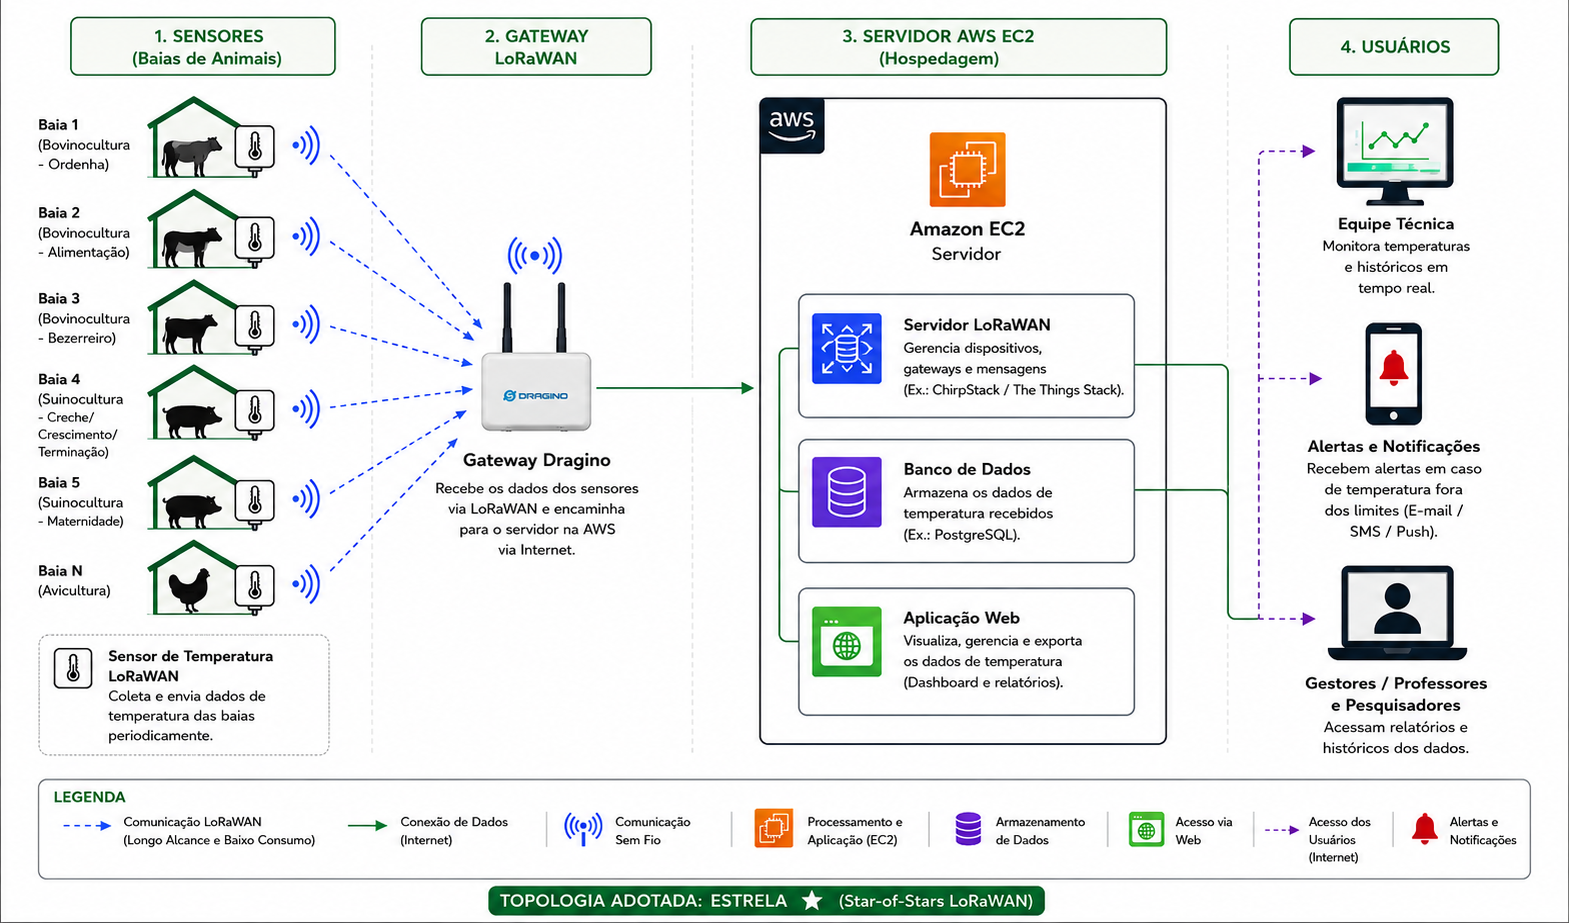
\includegraphics[width=\textwidth]{figuras/arquitetura_aws_sem_titulo.png}
\caption{Arquitetura da rede LoRaWAN e dos serviços de monitoramento.}
\label{fig:arquitetura}
\end{figure*}

A distribuição física originalmente definida é reproduzida na
Figura~\ref{fig:mapeamento}. Os seis pontos abrangem três ambientes da
bovinocultura, dois da suinocultura e um da avicultura. A Fábrica de Software foi
selecionada como ponto concentrador por dispor de energia, conectividade IP e
suporte técnico. Além de documentar a origem das escolhas, o mapa evidencia uma
vantagem central da tecnologia: conectar instalações dispersas sem lançar cabos
de dados entre os setores.

\begin{figure*}[t]
\centering
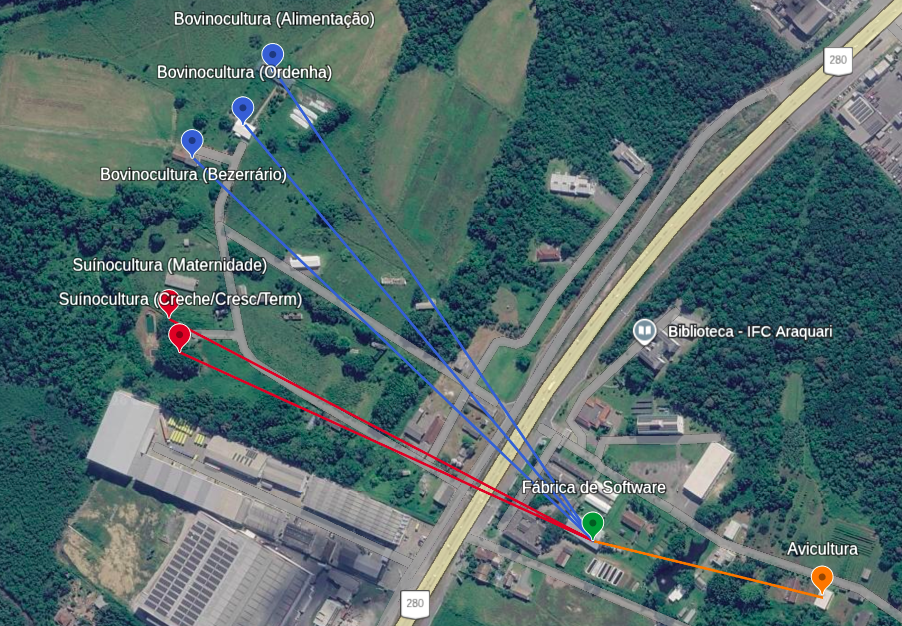
\includegraphics[width=0.94\textwidth]{figuras/mapeamento-000.png}
\caption{Mapeamento original dos pontos de monitoramento e do gateway no IFC
Campus Araquari.}
\label{fig:mapeamento}
\end{figure*}

O sensor mede a variável, forma uma carga útil compacta e transmite em intervalo
configurável. Depois da validação LoRaWAN, a aplicação associa a mensagem ao
setor e ao dispositivo, converte os valores, registra data e hora e compara a
medição com limites definidos pelos responsáveis. Uma condição fora do intervalo
gera evento de alerta; os valores permanecem disponíveis para consultas e
gráficos históricos.

\subsection{Componentes}

A Tabela~\ref{tab:componentes} resume os elementos principais definidos no
memorial. O LHT65N-DC opera como dispositivo Classe A, possui invólucro IP65 e
faixa declarada de medição de $-40$ a \SI{85}{\celsius}, com precisão aproximada
de $\pm\SI{0.3}{\celsius}$, conforme a especificação adotada no projeto. O
gateway LPS8N oferece oito canais LoRa e \textit{backhaul} IP. A quantidade de seis sensores foi
adotada para dois pontos representativos por setor, sujeita a ajuste após o
levantamento definitivo de propagação.

\begin{table*}[t]
\centering
\caption{Componentes principais da solução.}
\label{tab:componentes}
\begin{tabularx}{\textwidth}{@{}p{3.0cm}p{3.1cm}X@{}}
\toprule
\textbf{Camada} & \textbf{Componente} & \textbf{Função} \\
\midrule
Sensoriamento & 6 Dragino LHT65N-DC & Medir temperatura e, quando aplicável,
umidade; transmitir por LoRaWAN Classe A. \\
Acesso & Dragino LPS8N & Receber mensagens em \SI{915}{\mega\hertz} e
encaminhá-las à rede IP. \\
Rede/aplicação & AWS IoT Core, IoT Rules e aplicação web & Autenticar
dispositivos, gerenciar mensagens, aplicar regras e expor serviços. \\
Dados & Amazon DynamoDB e Amazon RDS & Preservar dados brutos e armazenar
medições processadas, dispositivos, setores, limites e alertas. \\
Operação e segurança & Amazon S3, CloudWatch e IAM & Manter arquivos e backups,
acompanhar métricas e controlar permissões. \\
\bottomrule
\end{tabularx}
\end{table*}

\subsection{Segurança, endereçamento e operação}

Cada dispositivo deve possuir identificadores e chaves únicos. Recomenda-se
ativação por \textit{over-the-air} (OTAA), armazenamento protegido das chaves e
separação entre as credenciais dos sensores, do banco e da aplicação. A
comunicação web deve empregar HTTPS, controle de acesso por perfil e registros de
auditoria. Backups periódicos e monitoramento dos serviços reduzem o impacto de
falhas da nuvem.

O gateway deve ser instalado em posição elevada, protegido e próximo a um ponto
de energia e conectividade. Os sensores devem ficar em estruturas fixas, longe de
impactos, chuva direta, fontes localizadas de calor e locais que produzam
medições não representativas. A altura e o abrigo precisam ser padronizados para
permitir comparação entre setores.

\section{Resultados do projeto e discussão}

\subsection{Qualidades e vantagens da solução}

A principal qualidade da solução é a adequação entre a tecnologia e o ambiente.
O LoRaWAN combina baixo consumo, alcance superior ao de redes locais
convencionais e tráfego compatível com mensagens periódicas de poucos bytes. Os
sensores alimentados por bateria dispensam pontos elétricos junto às baias, e a
comunicação sem fio reduz intervenções na infraestrutura física do campus. A
topologia permite incluir novos sensores sem alterar o caminho dos dispositivos
já instalados.

A centralização das medições transforma observações isoladas em séries
históricas comparáveis. Para os responsáveis pelos setores, isso pode antecipar
a identificação de temperaturas fora dos limites e orientar inspeções. Para
docentes e pesquisadores, a base temporal pode apoiar aulas práticas, estudos
ambientais e correlações com manejo e produtividade. Para a instituição, uma
infraestrutura comum evita soluções independentes em cada setor e favorece o
reaproveitamento do gateway e dos serviços em nuvem.

Na camada computacional, a separação entre recepção, processamento,
armazenamento e apresentação melhora a rastreabilidade e permite ampliar cada
componente conforme a demanda. Serviços de arquivos, métricas e identidade
acrescentam backup, observabilidade e controle de acesso. Como contraponto, a
arquitetura em nuvem exige controle de custos, configuração cuidadosa de
permissões e documentação operacional.

A área máxima esperada de \SI{1}{\kilo\meter} é compatível com o propósito de uma
LPWAN e com resultados encontrados na literatura. Contudo, não constitui alcance
garantido. O estudo de \citeonline{fu2022}, por exemplo, obteve desempenho
elevado a \SI{604}{\meter}, enquanto \citeonline{ahmed2025} mostrou degradação
mesmo em distâncias menores sob vegetação. A instalação no campus deve, portanto,
usar RSSI, SNR e razão de entrega de pacotes como critérios de posicionamento do
gateway.

\subsection{Viabilidade econômica}

O orçamento acadêmico consolidado é apresentado na Tabela~\ref{tab:orcamento}.
A mão de obra foi contabilizada como atividade da disciplina e, por isso, não
recebeu valor financeiro. Essa premissa precisa ser revista em uma contratação
real, juntamente com impostos, frete, instalação, manutenção, reposição de
baterias e custos recorrentes de nuvem.

\begin{table*}[t]
\centering
\caption{Síntese do orçamento inicial do projeto.}
\label{tab:orcamento}
\begin{tabularx}{\textwidth}{@{}X S[table-format=2.0] S[table-format=4.2]@{}}
\toprule
\textbf{Item} & {\textbf{Quantidade}} & {\textbf{Total (R\$)}} \\
\midrule
Sensores LoRaWAN Dragino LHT65N-DC & 6 & 1470.00 \\
Gateway LoRaWAN Dragino LPS8N & 1 & 870.00 \\
Baterias de reposição & 6 & 210.00 \\
Fixação, cabos, antena e fonte & 1 & 187.00 \\
Servidor em nuvem por quatro meses & 4 & 480.00 \\
\midrule
\multicolumn{2}{r}{\textbf{Total informado nos artefatos}} & {\bfseries 2977.00} \\
\bottomrule
\end{tabularx}

\smallskip
\footnotesize Fonte: elaborado pela autora com base no orçamento do projeto.
Há divergência aritmética entre as parcelas detalhadas (R\$~3.217,00) e o
total informado (R\$~2.977,00); o orçamento deve ser reconciliado antes da
aquisição.
\end{table*}

A soma dos valores discriminados nos artefatos é R\$~3.217,00, ou R\$~240,00
acima do total declarado. O valor anual de nuvem e o custo de longo prazo também
devem ser separados do investimento inicial.

\subsection{Critérios de qualidade}

Os indicadores da Tabela~\ref{tab:indicadores} tornam as qualidades pretendidas
verificáveis e evitam que alcance, autonomia ou disponibilidade sejam tratados
como benefícios garantidos antes de medições no campus.

\begin{table*}[t]
\centering
\caption{Indicadores propostos para validação.}
\label{tab:indicadores}
\begin{tabularx}{\textwidth}{@{}p{3.2cm}p{2.5cm}X@{}}
\toprule
\textbf{Indicador} & \textbf{Meta} & \textbf{Medição} \\
\midrule
Cobertura dos pontos & 100\% & Confirmar recepção em todos os locais
definidos, com registro de RSSI e SNR. \\
Entrega de mensagens & $\geq 95\%$ & Comparar sequências transmitidas e
persistidas por sensor. \\
Disponibilidade da comunicação & $\geq 95\%$ & Calcular tempo com recepção
regular no período de teste. \\
Latência de disponibilização & $\leq 60$ s & Medir entre coleta e exibição na
interface. \\
Precisão das medições & $\geq 95\%$ de concordância & Comparar com termômetro
de referência calibrado. \\
Disponibilidade da aplicação & $\geq 95\%$ & Monitorar API, banco e interface. \\
Usabilidade & $\geq 90\%$ de aprovação & Aplicar questionário aos usuários de
teste. \\
\bottomrule
\end{tabularx}
\end{table*}

A razão de entrega de pacotes pode ser calculada por

\begin{equation}
\mathrm{PDR}(\%) =
\frac{N_{\mathrm{recebidas}}}{N_{\mathrm{enviadas}}}\times 100.
\end{equation}

RSSI, SNR, distância, obstáculos e latência devem acompanhar esse indicador para
explicar eventuais perdas e orientar o posicionamento dos gateways.

\subsection{Riscos e limitações}

Os riscos de maior impacto são atraso na aquisição, indisponibilidade dos
sensores, perda do enlace entre gateway e nuvem, falha da aplicação e erro no
servidor. Fornecedores alternativos, testes de bancada, \textit{buffer} local,
rotinas de backup, supervisão de serviços e documentação de recuperação são
respostas previstas no projeto.

A principal limitação deste artigo é a ausência de medições obtidas por uma
implantação física completa no campus. Consequentemente, cobertura, autonomia,
latência e precisão não podem ser afirmadas como resultados alcançados. Outra
limitação é que os limites térmicos de alerta não foram fixados: eles dependem da
espécie, idade, sistema de criação e orientação dos profissionais responsáveis.
Por fim, o orçamento representa preços levantados para o projeto acadêmico e
precisa de atualização no momento da compra.

\section{Conclusão}

Este artigo consolidou o projeto de uma infraestrutura LoRaWAN para monitorar
temperatura nas instalações de bovinocultura, suinocultura e avicultura do IFC
Campus Araquari. A solução integra seis sensores, gateway multicanal,
conectividade IP, serviços em nuvem, banco de dados e aplicação web, cobrindo o
fluxo entre aquisição, armazenamento, visualização e alertas.

A análise da literatura e dos artefatos indica que a arquitetura é coerente com
o baixo volume de dados, a distribuição espacial dos pontos e a necessidade de
baixo consumo. O projeto também oferece uma base objetiva de validação, com metas
para cobertura, entrega de mensagens, disponibilidade, latência, precisão e
usabilidade. A revisão, entretanto, identificou a necessidade de reconciliar a
planilha de custos e de tratar o alcance de \SI{1}{\kilo\meter} como expectativa,
não como desempenho comprovado.

As vantagens potenciais ultrapassam a simples substituição da leitura manual: a
solução pode ampliar a continuidade do acompanhamento, reduzir o tempo entre um
desvio e sua percepção, apoiar decisões com dados históricos e criar uma base
compartilhada para ensino e pesquisa. A mesma infraestrutura admite novos pontos
e outras variáveis ambientais, preservada a validação de cobertura, consumo e
custos. Assim, o principal resultado é uma arquitetura coerente, expansível e
orientada ao uso institucional, cujos ganhos quantitativos deverão ser
confirmados em operação.

\bibliography{referencias}

\end{document}
